\section{Capture}
\label{section:capture}

As seen before, acquisitions only capture a subset of the scene geometry and color, so multiple acquisitions are required. This problem can be partially solved by recording multiple acquisitions instead of once. Therefore, a capture is a collection of acquisitions of the same scene and it's goal is to contain data from all the scene, in order to create a proper reconstruction of the scene. However, this raises some challenges, on how to plan and execute the multitude of acquisitions and how to merge the data from all of the acquisitions.

\begin{figure}
    
    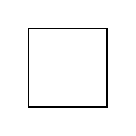
\begin{tikzpicture}
        
        \draw (0,0) rectangle (1, 1);

    \end{tikzpicture}

    \caption{Different positions of the 3D scanner affect the acquisition result}

    \label{figure:scene-acquisitions-example}

\end{figure}